\documentclass[12pt]{article}
\usepackage[T1]{fontenc}
\usepackage[T1]{polski}
\newcommand{\BibTeX}{{\sc Bib}\TeX}
\usepackage{graphicx}
\usepackage{amsmath} \usepackage{amssymb} \usepackage{amsfonts}
\usepackage[utf8]{inputenc}
\usepackage{minted}
\newcommand{\cljt}[1]{\mintinline{clojure}{#1}}
\usepackage{tikz-cd}
\setlength{\textheight}{21cm}

\title{{\bf Zadanie nr 1 - Generacja sygnału i szumu}\linebreak
	Cyfrowe Przetwarzanie Sygnałów}
\author{Jakub Mileczarek idk \and Imię Nazwisko, 236551}
\date{2023-03-06} % jak zdążymy xd

\begin{document}
\clearpage\maketitle
\thispagestyle{empty}
\newpage
\setcounter{page}{1}
\section{Cel zadania}
Celem zadania byłó zaimplementowanie programu pozwalającego na tworzenie i wyświetlanie sygnałów cyfrowych.
%Opis celu zadania (proszę nie przepisywać treści instrukcji!).\\
%Sprawozdanie należy wykonać na podstawie\\
%szablonu \LaTeX-owego \texttt{sprawozdanie-wzor.tex}.


%\section{Wstęp teoretyczny}

%Krótki opis wykorzystywanych metod~\cite{dowolna_etykieta_artykulu}. Proszę nie umieszczać ogólnie znanych z literatury
%wzorów oraz definicji. Należy podać jaka metoda została zastosowana, dlaczego oraz podać wykorzystaną literaturę (korzystając z odwołań do pozycji bibliografii~\cite{dowolna_etykieta_ksiazki}).\\
%Przygotowując bibliografię należy korzystać z podanego\\
%szablonu \BibTeX-owego \texttt{bibliografia-wzor.bib}.

%%%%%%%%%%%%%%%%%%%%%%%%%%%%%%%%%%%%%%%%%%%%%%%%%%%%%%%%%%%%%%%%%%%%%%%%%%%%%%%%%%%%%%%%%%%%%%%%%%%%%%%%%%%%%%%%%
% PODROZDZIA\xC5\x81 PT. ZALACZNIKI
%%%%%%%%%%%%%%%%%%%%%%%%%%%%%%%%%%%%%%%%%%%%%%%%%%%%%%%%%%%%%%%%%%%%%%%%%%%%%%%%%%%%%%%%%%%%%%%%%%%%%%%%%%%%%%%%%
\section{Wstęp}
zamiast programu z graficznym lub tekstowym interfejsem użytkownika zaimplementowaliśmy malutki, prosty w obsłudze język dziedzinowy.

\section{implementacja}
Program został zaimplementowany w \texttt{clojure}, funkcyjnym, lispopodobnym języku hostowanym na \texttt{JVM}. Do wykonania grafów użyliśmy biblioteki \texttt{incanter}, funkcję zwracającą wartość z rozkładem gaussowskim znaleźliśmy w bibliotece \text{cern.jet.random}, do wsparcia liczb złożonych wykorzystujemy wrapper \texttt{complex} do bibloteki \texttt{org.apache.commons.math3.complex}.
\subsection{reprezentacje}
Program korzysta wewnętrznie z 4 różnych reprezentacji sygnału:
\begin{itemize}
	\item		\cljt{:spec} \\
	      czytelny dla człowieka słownik zawierający specyfikację, większość elementów ma dość rozsądne wartości domyślne więc może być pominięta, n.p:\\
	      \cljt{{:function :triangle :fill 0.4 :amplitude 0.4}} \\
	      \cljt{{:function :sin :phase 0.3 :duration 3}} \\
	      dla wygody niektóre klucze posiadają skrócone wersje: \\
	      \cljt{{:f :sin :A 2 :p 3 :s 2 :e 5}}

	\item		\cljt{:fancy} \\
	      reprezentacja sygnału ciągłego jako słownik zawierający informacje o początku i końcu sygnału oraz funkcję zwracającą wartość sygnału w danym czasie
	\item		\cljt{:discrete} \\
	      zdyskretyzowana forma sygnału, zawiera informacje o częstotliwości próbkowania, offsecie, ilości próbek, i próbki
	\item		\cljt{:file} \\
	      nazwa pliku zawierającego sygnał
\end{itemize}
Funkcje do manipulacji wspierają jedynie \cljt{:discrete} i \cljt{:fancy} (nie wszystkie), inne reprezentacje są w miarę potrzeb konwertowane do którejś ze wspieranych form
\begin{figure}
	\[\begin{tikzcd}[%
				%row sep = 20mm, column sep = 20mm, % both optional, adapt as you please
				cells={},
				every arrow/.append style={shorten <= 1mm, shorten >= 1mm}] % both optional. Default connects the arrow directly to the circles
			:file \arrow[shift left]{r} &
			:discrete \arrow[shift left]{l} &
			:fancy \arrow{l} &
			:spec \arrow{l} &
		\end{tikzcd}\]
	\caption{różne reprezentacje i konwersje między nimi}
\end{figure}

Dodatkowym i być może nieoczekiwanym krokiem jest \cljt{:fancy}, jego celem jest maksymalne opóźnienie próbkowania, tak by można było np. dodać do sygnału z pliku sumę dwóch sygnałów, i spróbkowanie ich dopiero w momencie w którym znana jest jego częstotliwość próbkowania.

\subsection{częstotliwość}
Program stara się zachować częstotliwość sygnału, by przy tworzeniu histogramu uciąć wystającą część okresu. w przypadku wykonywania opreracji na sygnale częstotliwość sygnału wynikowego jest najmniejszą wspólną wielokrotnością sygnałów stanowiących argumenty operaji.
\section{Instrukcja}
\subsection{wprowadzanie sygnałów}
Użytkownik wprowadza sygnały (poza impulsem jednostkowym) w formie \cljt{:spec} poprzez mapę zawierającą
chciane parametry
\begin{itemize}
	\item \cljt{:function, :fun, :fn, :f} -- jedno z słów kluczowych oznaczających funkcje
	      \begin{itemize}
		      \item \cljt{:sin} sinusoida
		      \item \cljt{:sin-half} sinusoida wyprostowana jednopołówkowo
		      \item \cljt{:sin-double} sinusoida wyprostowana dwupołuwkowo
		      \item \cljt{:square} sygnał prostokątny (\cljt{:fill} -- stopień wypełnienia)
		      \item \cljt{:square-sym} sygnał prostokątny symetryczny
		      \item \cljt{:triangle} sygnał trójkątny (\cljt{:fill} -- część okresu przeznaczona na zbocze narastające)
		      \item \cljt{:jump} skok jednostkowy (\cljt{:fill} -- czas skoku)
		      \item \cljt{:noise} szum (-1 -- 1)
		      \item \cljt{:noise-gauss} szum gaussowski
		      \item \cljt{:noise-impulse} szum impulsowy (\cljt{:fill} -- prawdopodobieństwo)
	      \end{itemize}
	\item \cljt{:period, :per, :p} -- okres, wartość domyślna = 1
	\item \cljt{:amplitude :amp :a :A} -- amplituda, wartość domyślna = 1
	\item \cljt{:fill} -- znaczenie różne w zależności od funkcji, domyślnie 0.5

	\item \cljt{:phase, :ph} -- przesunięcie fazowe, domyślnie 0.0

	\item \cljt{:start, :s} -- czas początku, wyrażony w sekundach, domyślnie 0
	\item \cljt{:duration, :d, :l} -- czas trwania, wyrażony w sekundach, domyślnie 5
	\item \cljt{:end, :e} -- koniec, bez wartości domyślnej, jeżeli podany, jest brany pod uwagę zamiast \cljt{:duration}
\end{itemize}
Do wprowadzania impulsu jednostkowego służy funkcja \cljt{impulse} biorąca jako parametry \cljt{:A} --amplituda, domyślnie 1.0, \cljt{:A} --amplituda, domyślnie 1.0, sampling, domyślnie 1/1000,  \cljt{:ns} -- nr. próbki (liczony od 0) w której występuje impuls. przykład \cljt{(impulse :ns 5 :A 2.0)}
\subsection{operacje}
Do przesuwania sygnałów w czasie służy funkcja \cljt{(tshift x t)}, gdzie \cljt{x} to sygnał a \cljt{t} to czas. \\
Do operacji na sygnale służą funkcje \cljt{fop, dop}, pierwsza z nich działa na sygnałach typu \cljt{:fancy}, a druga na \cljt{:discrete}, automatycznie próbkując inne sygnały z odpowiednią częstotliwością. Sygnatura obu z nich jest taka sam \cljt{(fop funkcja sygnał1 sygnał2 sygnałn)}, \cljt{funkcja} musi zostanie wywołana z wartościami poszczególnych sygnałów w danym czasie. przykłady: \\
\cljt{(dop - "sygnał" {:fun :sin :d 1})} -- wczyta sygnał z pliku, dokona dyskretyzacji funkcji sinus na przedziale od 0 do 1 z częstotliwością taką samą jak ta wczytana z pliku, i dla każdej pary próbek wykona operację odejmowania, zwróci \cljt{:discrete} \\
\cljt{(fop * {:fun :sin} {:fun :sin :period 1/3})} -- zwróci sygnał w postaci \cljt{:fancy} którego wartości w poszczególnych chwilach czasowych zostaną obliczone później
\subsection{próbkowanie}
domyślna częstotliwość próbkowania jest zmienną dynamiczną, jej wartość można ustawić poprzez \\
\cljt{(binding [sampling-frequency 1/20)] kod)))}

\subsection{prezentacja}
Funkcje znajdujące się w przestrzeni nazw \cljt{graph}
\begin{itemize}
	\item \cljt{show} -- wyświetl sygnał jako punkty lub krzywą w zależności od typu sygnału
	\item \cljt{histogram} -- wyświetla histogram sygnału dyskretnego
	\item \cljt{stat} -- zwraca mapę zawierającą parametry sygnału dyskretnego
\end{itemize}

\subsection{zapisywanie i wczytywanie sygnałów do pliku}
Do zapisywania sygnału do pliku służy procedura \cljt{write} biorąca dwa argumenty, nazwę pliku i sygnał;
\cljt{(write "sygnał" {:function :sin})}
wczytywanie odbywa się automatycznie;
\cljt{(show (fop + "sygnał" {:function :square}))}.
\section{wnioski}

Nasz program pozwala na dość łatwe i powtarzalne tworzenie sygnałów.

\begin{figure}[H]
	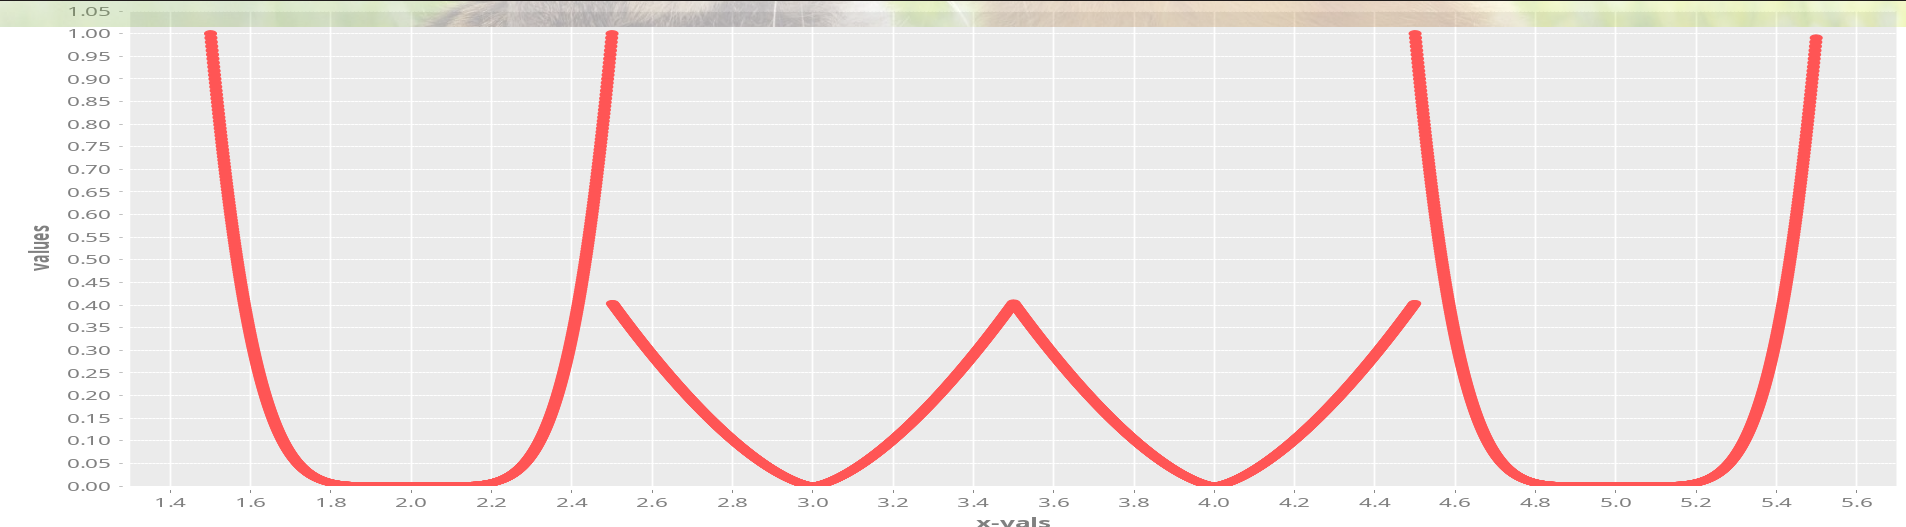
\includegraphics[width=\linewidth]{uwu.png}
	\caption{graf funkcji $UwU(x)$}
\end{figure}

%%%%%%%%%%%%%%%%%%%%%%%%%%%%%%%%%%%%%%%%%%%%%%%%%%%%%%%%%%%%%%%%%%%%%%%%%%%%%%%%%%%%%%%%%%%%%%%%%%%%%%%%%%%%%%%%%
% BIBLIOGRAFIA
%%%%%%%%%%%%%%%%%%%%%%%%%%%%%%%%%%%%%%%%%%%%%%%%%%%%%%%%%%%%%%%%%%%%%%%%%%%%%%%%%%%%%%%%%%%%%%%%%%%%%%%%%%%%%%%%%

\renewcommand\refname{Bibliografia}
\bibliographystyle{plain}
%\bibliography{bibliografia_wzor}

\end{document}
